\documentclass{minimal}
\usepackage[a4paper,margin=1cm,landscape]{geometry}
\usepackage{tikz}
\usetikzlibrary{positioning,shadows,arrows}

\begin{document}
\begin{center}
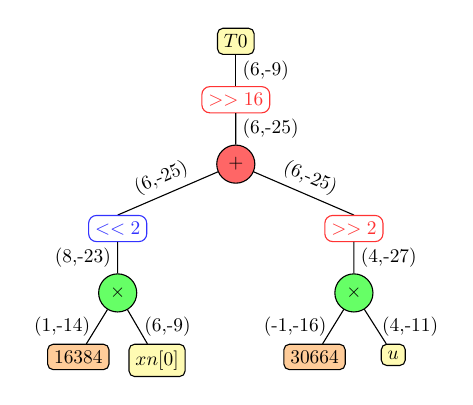
\begin{tikzpicture}[
     dec1/.style={rectangle, draw=red!80, rounded corners=1mm, fill=white,
        text centered, anchor=north, text=red!80, scale = 0.7},
    dec2/.style={rectangle, draw=blue!80, rounded corners=1mm, fill=white,
        text centered, anchor=north, text=blue!80, scale = 0.7},
    adder/.style={circle, draw, fill=red!60,
        text centered, anchor=north, text=black, scale = 0.7},
    mult/.style={circle, draw, fill=green!60,
        text centered, anchor=north, text=black, scale = 0.7},
     cst/.style={rectangle, rounded corners=0.7mm, draw, fill=orange!40,
        text centered, anchor=north, text=black, scale = 0.7},
     var/.style={rectangle, rounded corners=0.7mm, draw, fill=yellow!30,
        text centered, anchor=north, text=black, scale = 0.7},
     fpr/.style = {scale = 0.7},
    level distance=0.4cm, growth parent anchor=south
]
\node (Sortie) [var] {$T0$}
child{[sibling distance=3.000000cm]
	node(DAdd_0) [dec1] {$>>16 $}
	child{
		node(Add_0) [adder] {$+$}
	child{[sibling distance=1cm]
		node(DMultxn0 gamma  23) [dec2] {$<<2 $}
		child{
			node(Multxn0 gamma  23) [mult] {$\times$}
			child{
				node(Cst0) [cst] {16384}
			edge from parent node[fpr, left] {(1,-14)}
			}
			child{
				node(Var0) [var] {$xn[0]$}
			edge from parent node[fpr, right] {(6,-9)}
			}
			edge from parent node[fpr, left] {(8,-23)}
		}
		edge from parent node[fpr, left,sloped,above] {(6,-25)}
	}
	child{[sibling distance=1cm]
		node(DMultu gamma  27) [dec1] {$>>2 $}
		child{
			node(Multu gamma  27) [mult] {$\times$}
			child{
				node(Cst1) [cst] {30664}
			edge from parent node[fpr, left] {(-1,-16)}
			}
			child{
				node(Var1) [var] {$u$}
			edge from parent node[fpr, right] {(4,-11)}
			}
			edge from parent node[fpr, right] {(4,-27)}
		}
		edge from parent node[fpr, right,sloped,above] {(6,-25)}
	}
		edge from parent node[fpr, right] {(6,-25)}	}
	edge from parent node[fpr, right] {(6,-9)}
}

;
        
\end{tikzpicture}
\end{center}
\end{document}